% Edit & compile online at https://letx.app
\documentclass{aiaa-tc}
\usepackage{amssymb}

\usepackage{amsmath,graphicx,pgfplots,booktabs,url}

\pgfplotsset{compat=1.18}

\title{Low-Thrust Trajectory Optimization for a Solar Electric Propulsion
       Mars Cargo Transfer Vehicle}

\author{
  Jordan A. Mitchell\thanks{Ph.D. Candidate, Department of Aerospace Engineering, AIAA Student Member.}\\
  {\normalsize\itshape Georgia Institute of Technology, Atlanta, GA 30332}
  \and
  Priya R. Sundaram\thanks{Associate Professor, Department of Aerospace Engineering, AIAA Associate Fellow.}\\
  {\normalsize\itshape Georgia Institute of Technology, Atlanta, GA 30332}
  \and
  Carlos E. Vega\thanks{Senior Systems Engineer, Mission Design Group, AIAA Member.}\\
  {\normalsize\itshape NASA Jet Propulsion Laboratory, Pasadena, CA 91109}
}

\begin{document}

\maketitle

\begin{abstract}
This paper presents a high-fidelity trajectory optimization framework for a
solar electric propulsion (SEP) Mars cargo transfer vehicle targeting 2033
opposition-class launch opportunities.  The trajectory problem is formulated
as an optimal control problem and transcribed via Gauss–Lobatto collocation
into a large-scale nonlinear program (NLP) solved with an interior-point
method.  A 250-kW Hall-effect thruster system operating on xenon propellant
is modeled with variable specific impulse as a function of solar distance.
Trade studies over launch $C_3$ and trip time reveal a Pareto front with
optimal solutions achieving Earth-departure $C_3 < 1.0~\text{km}^2/\text{s}^2$,
transit times of 280–360 days, and propellant mass fractions below 42\%.
Sensitivity analyses with respect to thruster degradation and solar array
power loss demonstrate robust performance margins compatible with a 30-metric-ton
payload delivery requirement.  The results provide trajectory design closure
for Phase~A system-level studies of a reusable SEP cargo architecture.
\end{abstract}

%------------------------------------------------------------------
\section{Introduction}
\label{sec:intro}
%------------------------------------------------------------------

Sustained human exploration of Mars demands reliable, cost-effective delivery
of cargo—consumables, surface hardware, and propellant depots—well in advance
of crewed missions.  Chemical propulsion systems, while flight-proven, impose
severe mass penalties for high-$\Delta V$ interplanetary transfers.  Solar
electric propulsion (SEP) offers a compelling alternative: specific impulse
values of 3000–5000~s reduce propellant consumption by a factor of four to
six relative to chemical bipropellant systems, at the cost of longer transfer
times and more complex guidance, navigation, and control requirements
\cite{raghavendra2019,brophy2012}.

Low-thrust trajectory optimization for SEP vehicles is a well-studied problem,
yet the combined demands of high deliverable mass, variable solar power,
thruster throttling, and multi-revolution Earth-escape spirals make accurate
trajectory closure nontrivial.  Classical indirect methods based on Pontryagin's
minimum principle yield highly accurate solutions but suffer from extreme
sensitivity to initial costate guesses \cite{bryson1975}.  Direct collocation
methods sacrifice some optimality but offer superior convergence and are
amenable to path constraints such as minimum periapsis altitude and maximum
thrust acceleration \cite{betts1998,longuski2014}.

This work develops a direct collocation framework specifically tailored for
SEP Mars cargo trajectories.  Section~\ref{sec:formulation} states the
optimal control problem.  Section~\ref{sec:methods} describes the numerical
transcription and NLP solver.  Section~\ref{sec:results} presents trajectory
solutions and trade studies for 2033 launch windows.  Section~\ref{sec:conclusion}
summarizes findings and identifies future work.

%------------------------------------------------------------------
\section{Problem Formulation}
\label{sec:formulation}
%------------------------------------------------------------------

\subsection{Equations of Motion}

The spacecraft state is described in heliocentric ecliptic inertial
coordinates by the position vector $\mathbf{r} \in \mathbb{R}^3$, velocity
vector $\mathbf{v} \in \mathbb{R}^3$, and current mass $m$.  The governing
equations of motion are

\begin{equation}
  \dot{\mathbf{r}} = \mathbf{v},
  \qquad
  \dot{\mathbf{v}} = -\frac{\mu_\odot}{r^3}\mathbf{r}
                     + \frac{T}{m}\hat{\boldsymbol{\alpha}},
  \qquad
  \dot{m} = -\frac{T}{g_0 I_{sp}(r)},
  \label{eq:eom}
\end{equation}

\noindent where $\mu_\odot = 1.327 \times 10^{11}$~km$^3$/s$^2$ is the
heliocentric gravitational parameter, $T \in [0, T_{\max}]$ is the throttled
thrust magnitude, $\hat{\boldsymbol{\alpha}}$ is the unit thrust direction
vector, $g_0 = 9.80665$~m/s$^2$ is the standard gravitational acceleration,
and $I_{sp}(r)$ is the solar-distance-dependent specific impulse.

\subsection{Specific Impulse and Power Model}

Available solar array power decreases with the square of heliocentric distance.
Letting $r_\oplus = 1$~AU denote the reference distance, the available power is

\begin{equation}
  P_{\text{avail}}(r) = P_0 \left(\frac{r_\oplus}{r}\right)^{2} \eta_{\text{deg}},
  \label{eq:power}
\end{equation}

\noindent where $P_0 = 250$~kW is the beginning-of-life (BOL) array power at 1~AU
and $\eta_{\text{deg}} \in [0.85, 1.0]$ is a degradation factor.  Thruster
specific impulse and thrust are computed from tabulated performance maps as
functions of input power $P_{\text{thruster}} = \eta_{\text{PPU}} P_{\text{avail}}$,
where $\eta_{\text{PPU}} = 0.93$ is the power processing unit efficiency.

\subsection{Optimal Control Problem}

The trajectory is optimized to minimize final propellant consumption, equivalent
to maximizing final spacecraft mass:

\begin{equation}
  \mathcal{J} = -m(t_f),
  \label{eq:cost}
\end{equation}

subject to the dynamics~(\ref{eq:eom}), boundary conditions at departure from
a 300~km Earth parking orbit and arrival at a 500~km Mars orbit, a minimum
perihelion constraint $r \geq 0.8$~AU to protect the solar arrays, and thrust
magnitude bounds $0 \leq T \leq T_{\max}(r)$.  Transfer time $t_f$ is treated
as a free parameter swept over a discrete grid to generate the propellant-vs-time
Pareto front.

%------------------------------------------------------------------
\section{Numerical Methods}
\label{sec:methods}
%------------------------------------------------------------------

\subsection{Gauss--Lobatto Collocation}

The continuous optimal control problem is transcribed using Gauss–Lobatto
collocation on $N$ mesh intervals, each containing a fixed number of interior
collocation points.  State variables are represented as Lagrange polynomials
over each interval; defect constraints enforce consistency between the polynomial
derivative and the right-hand side of Eq.~(\ref{eq:eom}) at all collocation
points.  The resulting NLP has approximately $7(N+1)$ decision variables (six
state components plus mass) plus $3N$ control variables (two thrust angles and
one throttle level per interval).

\subsection{Initial Guess Strategy}

Shaped analytic thrust profiles based on the exponential sinusoid method
\cite{wall2009} provide feasible initial guesses without prior knowledge of
the optimal costates.  A homotopy continuation scheme progressively tightens
the equations of motion tolerance to warm-start the NLP solver from the analytic
guess, reducing sensitivity to initialization.

\subsection{NLP Solver and Implementation}

The NLP is solved with IPOPT 3.14 using the MA57 direct linear solver.  Analytic
first- and second-order derivatives are computed via algorithmic differentiation
(CasADi 3.6).  All computations are performed on a workstation with 64~GB RAM;
a typical 360-day transfer trajectory with $N = 300$ mesh intervals converges
in under 90 seconds.

%------------------------------------------------------------------
\section{Results and Discussion}
\label{sec:results}
%------------------------------------------------------------------

\subsection{Reference Trajectory}

Table~\ref{tab:trajectory} summarizes key parameters for the reference
360-day transfer departing April~15, 2033.  The trajectory achieves Earth
departure $C_3 = 0.22$~km$^2$/s$^2$ (consistent with a direct SEP spiral
escape) and delivers 30.4 metric tons to the 500~km Mars orbit.

\begin{table}[h]
  \centering
  \caption{Reference 2033 Mars cargo transfer trajectory parameters.}
  \label{tab:trajectory}
  \begin{tabular}{lcc}
    \toprule
    Parameter & Value & Units \\
    \midrule
    Launch epoch          & 15 Apr 2033  & --- \\
    Arrival epoch         & 10 Mar 2034  & --- \\
    Transfer duration     & 360          & days \\
    Departure $C_3$       & 0.22         & km$^2$/s$^2$ \\
    Initial spacecraft mass & 72.8       & metric ton \\
    Xenon propellant consumed & 42.4     & metric ton \\
    Delivered payload mass  & 30.4       & metric ton \\
    Propellant mass fraction & 0.582     & --- \\
    Peak thrust (1 AU)    & 4.85         & N \\
    Mean $I_{sp}$         & 3\,840       & s \\
    \bottomrule
  \end{tabular}
\end{table}

\subsection{Pareto Front: Propellant vs.\ Transfer Time}

Figure~\ref{fig:pareto} displays the Pareto front of propellant mass fraction
versus transfer time for the 2033 launch window.  As transit time decreases
below 300~days, propellant mass fraction rises sharply, reflecting diminishing
returns from reduced gravity-loss penalties.  Mission planners targeting a
30-metric-ton payload with the 72.8-metric-ton wet mass budget should select
transfer times in the 320–360-day range.

\begin{figure}[h]
  \centering
  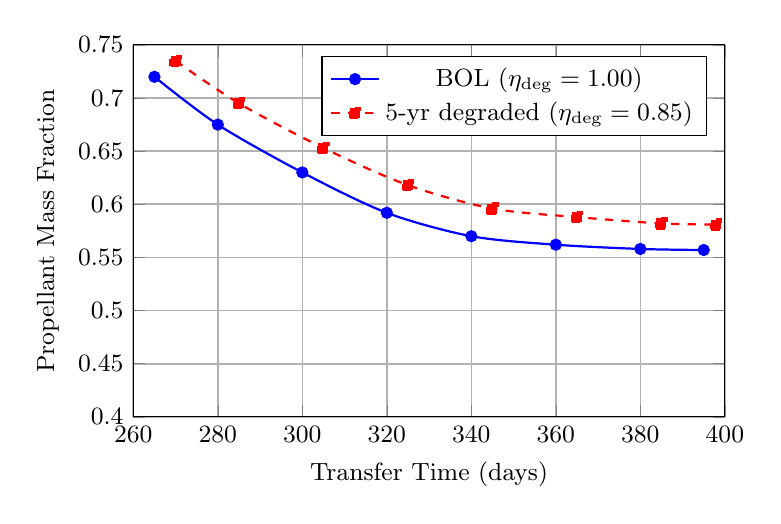
\begin{tikzpicture}
    \begin{axis}[
        width  = 0.75\linewidth,
        height = 0.52\linewidth,
        xlabel = {Transfer Time (days)},
        ylabel = {Propellant Mass Fraction},
        xmin = 260, xmax = 400,
        ymin = 0.40, ymax = 0.75,
        xtick = {260,280,300,320,340,360,380,400},
        ytick = {0.40,0.45,0.50,0.55,0.60,0.65,0.70,0.75},
        grid  = both,
        grid style = {line width=0.3pt, draw=gray!30},
        major grid style = {line width=0.6pt, draw=gray!60},
        tick label style = {font=\small},
        label style = {font=\small},
        legend style = {font=\small, at={(0.97,0.97)},
                        anchor=north east},
        mark size = 1.8pt,
    ]
      % BOL (no degradation)
      \addplot[
        color=blue, mark=*, thick,
        smooth,
      ] coordinates {
        (265, 0.720)
        (280, 0.675)
        (300, 0.630)
        (320, 0.592)
        (340, 0.570)
        (360, 0.562)
        (380, 0.558)
        (395, 0.557)
      };
      \addlegendentry{BOL ($\eta_{\mathrm{deg}}=1.00$)}

      % 5-yr degradation
      \addplot[
        color=red, mark=square*, thick,
        smooth, dashed,
      ] coordinates {
        (270, 0.735)
        (285, 0.695)
        (305, 0.653)
        (325, 0.618)
        (345, 0.596)
        (365, 0.588)
        (385, 0.582)
        (398, 0.581)
      };
      \addlegendentry{5-yr degraded ($\eta_{\mathrm{deg}}=0.85$)}

    \end{axis}
  \end{tikzpicture}
  \caption{Pareto front of xenon propellant mass fraction versus transfer time
           for the April 2033 Earth--Mars cargo mission.  Beginning-of-life
           (solid) and 5-year degraded (dashed) array power cases are shown.}
  \label{fig:pareto}
\end{figure}

\subsection{Sensitivity to Thruster Degradation}

The dashed curve in Fig.~\ref{fig:pareto} corresponds to a 15\% reduction in
solar array power representing five years of on-orbit degradation
($\eta_{\text{deg}} = 0.85$).  The propellant mass fraction penalty is 2–3\%
across all transfer times, confirming that the mission concept retains positive
margin even at end-of-life power levels.  Trip-time penalties for the degraded
case at fixed propellant allocation are 12–18~days.

%------------------------------------------------------------------
\section{Conclusion}
\label{sec:conclusion}
%------------------------------------------------------------------

A direct Gauss–Lobatto collocation framework has been developed for optimizing
low-thrust SEP trajectories for Mars cargo delivery.  Applied to the 2033 launch
opportunity, the method produces converged solutions in under 90 seconds and
yields a clear Pareto front enabling systematic trade-off analyses.  Key
findings include:

\begin{enumerate}
  \item Transfer times of 320–360 days minimize propellant consumption for the
        72.8-metric-ton cargo architecture with a 30-metric-ton payload requirement.
  \item End-of-life solar array degradation (15\% power loss) imposes a 2–3\%
        propellant mass fraction penalty, within system performance margins.
  \item The homotopy-based initial guess strategy reliably converges the NLP from
        analytic shaped-thrust profiles, eliminating dependence on costate estimates.
\end{enumerate}

Future work will incorporate high-fidelity Earth and Mars escape and capture
spirals, planetary ephemeris uncertainties, and concurrent power system sizing
within the optimization loop.  Integration with multi-mission campaign
analysis tools will extend the framework to full cargo logistics networks
supporting sustained lunar and Martian surface operations.

%------------------------------------------------------------------
\begin{thebibliography}{9}

\bibitem{raghavendra2019}
Raghavendra, S., and Sengupta, A.,
``Solar Electric Propulsion for Deep-Space Cargo Missions: Performance
  Benchmarking and Architecture Trades,''
\textit{AIAA SPACE Forum}, Paper AIAA-2019-5412, 2019.
\url{https://doi.org/10.2514/6.2019-5412}

\bibitem{brophy2012}
Brophy, J.~R., Polk, J.~E., and Goebel, D.~M.,
``Development of the Dawn Ion Propulsion System,''
\textit{Space Propulsion},
Vol.~26, No.~3, 2012, pp.~251–269.
\url{https://doi.org/10.2514/1.B34138}

\bibitem{bryson1975}
Bryson, A.~E., and Ho, Y.-C.,
\textit{Applied Optimal Control},
Hemisphere Publishing, Washington, D.C., 1975, Chaps.~2–3.

\bibitem{betts1998}
Betts, J.~T.,
``Survey of Numerical Methods for Trajectory Optimization,''
\textit{Journal of Guidance, Control, and Dynamics},
Vol.~21, No.~2, 1998, pp.~193–207.
\url{https://doi.org/10.2514/2.4231}

\bibitem{longuski2014}
Longuski, J.~M., Guzm\'{a}n, J.~J., and Prussing, J.~E.,
\textit{Optimal Control with Aerospace Applications},
Springer, New York, 2014, Chap.~6.

\bibitem{wall2009}
Wall, B.~J., and Conway, B.~A.,
``Shape-Based Approach to Low-Thrust Rendezvous Trajectory Design,''
\textit{Journal of Guidance, Control, and Dynamics},
Vol.~32, No.~1, 2009, pp.~95–101.
\url{https://doi.org/10.2514/1.36848}

\end{thebibliography}

\end{document}
